\section{Real Time Operating System}

Responds to events within a strictly defined time.
The scheduler is deterministic, meaning that the time it takes to switch between tasks is predictable.
Priority based scheduling is used to determine which task to run next. Thread=task.
Data is processed as it comes in, typically without buffer delays.

Application of RTOS could be airbag deployment, anti-lock braking system, etc.

\textbf{FreeRTOS}

RTOS small enough to run on a microcontroller. Embedded controllers don't warrant full RTOS
because of their hardware limitation. FreeROTS provides only:

\begin{itemize}
	\item Real-time scheduling functionality
	\item Inter-task communication
	\item Timing and synchronization primitives
\end{itemize}

\textbf{Multi-tasking}

Kernel - core of OS.

Multi-tasking in OS is if the OS can run multiple tasks at the same time.
This allows for complex applications to be subdivided into small tasks.

\begin{center}
	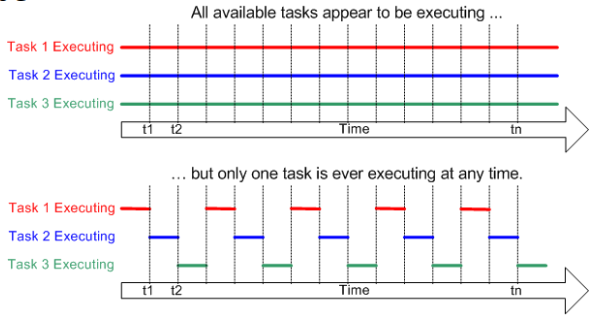
\includegraphics[width=0.6\textwidth]{images/multitasking.png}
\end{center}

\textbf{Scheuler}

The scheduler is a part of the kernel that decides which task will be executed when.
The scheduler can suspend and resume tasks, but tasks can suspend themselves too.

\textbf{FreeRTOS choice of scheduling policy}

Two choices: Preemptive and Cooperative. Pre-emptive always runs the highest priority task that is ready to run.
Having multiple tasks with the same priority, they will run using round robin scheduling.
Co-operative scheduling is where context switches only occur if a task blocks or explicitly calls task YIELD().

\newpage

\textbf{FreeRTOS Task States}

There are four states in FreeRTOS:
Running, Ready, Blocked, Suspended.
Running is the task that is currently executing.
Ready is where the task is able to execute but is not currently executing due to another task with equal or higher priority running.
Blocked is where the task waits for a temporal or external event. It can block waiting for a queue or semaphore event.
Suspended is where the task is not available for scheduling. Tasks only enter or exit suspend by vTaskSuspend() and xTaskResume().

\begin{center}
	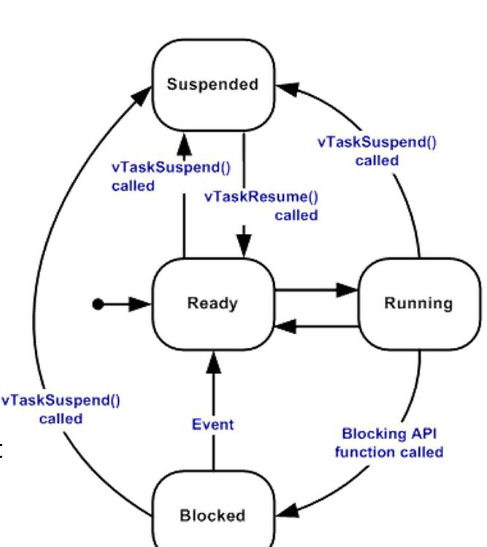
\includegraphics[width=0.4\textwidth]{images/freeStates.png}
\end{center}

\textbf{Sempahores}

Semaphores are used to synchronize tasks and protect shared resources.
A semaphore can be a signaling semaphore or a mutex.
Meaning that a semaphore can be used to signal between tasks or to lock a resource.
Semaphores can be binary or counting.

\textbf{Resource Management}

There is a potential risk for a conflict in a multitasking system. If one task starts to access a resource
but does not complete its access before being transitioned out of the running state. If the task left the resource
in an inconsistent state, then access to the same resource by any other task or interrupt could result in data corruption.

\textbf{Mutual exclusion}

Mutual exclusion can be implemented in FreeRTOS by: Disabling interrupts, using a mutex or disabling the scheduler.

\textbf{Mutex}

A mutex is a special type of binary semaphore that is used to control access to a resource.
Mutex vs. Semaphore: Mutexes can be released only by the task which took them, while binary semaphores can be released
by any task. Mutexes are for protecting resources - binary semaphores are for serialization and signaling.




